% !TeX spellcheck = en_US
\section{Problem 7}
A continuous piecewise linear function is a function that is linear on every segment of its domain.\\
To show that a Multi-Layer Perceptron (MLP) using only the ReLU (Rectified Linear Unit) or pReLU (Parametric Rectified Linear Unit) activation functions constructs a continuous linear function, we must first review the properties of these activation functions. \\

Let’s consider the ReLU activation function for this explanation.

The ReLU activation function is defined as:\\
\begin{equation}
	\operatorname{ReLU}(x)=\operatorname*{max}(x,0)={\left\{\begin{array}{ll}
			{x}&{{\mathrm{if~}}x>0,}\\ 
			{0}&{{\mathrm{otherwise,}}}
			\end{array}\right.}		
\end{equation}

We need to check if they meet the prerequisites of continuity and linearity.
\begin{itemize}
	\item \underline{Is it Continuous?}\\
	Yes it is, because it has no break points for the various values of $x$
	\item \underline{Is it Linear?}\\
	Yes it is, because it consists of only two linear parts. ReLU is linear within its segments.
\end{itemize}

In an MLP, the output of each neuron is computed by applying an affine transformation (multiplying the weights and adding the bias), followed by ReLU activation. The key property of ReLU activation is that it is a piecewise linear function.
When you consider a single neuron with ReLU activation, it essentially performs two operations:
\begin{enumerate}
	\item For inputs $x$ where $x > 0$, the output is $x$.
	\item For inputs $x$ where $x \leq 0$, the output is $0$
\end{enumerate}

Having a closer look, the first operation $(x > 0)$ is a linear transformation with a slope of $1$ (output is $y = x$), and the second operation $(x \leq 0)$ is a constant zero (output is $y = 0$).\\

By composing several such neurons in an MLP architecture, we effectively create a composition of linear transformations and constant zeros. Since the operations of the individual ReLU neurons are piecewise linear, the combination of these operations is naturally also a piecewise linear function.\\
The breakpoints in the piecewise linear function occur where the activations of the neurons go from $0$ to the actual linear operation -when the input $x$ exceeds $0$ -. As you move from one layer to the next in the network, we are effectively combining multiple piecewise linear functions, resulting in a more complex piecewise linear function overall.\\

The activation function pReLU behaves similarly, but it introduces a learnable parameter $a$ for the negative slope that allows a continuous range of slopes for the linear part when $x$ is negative.\\

To summarize, an MLP that uses only ReLU (or pReLU) activation functions constructs a continuous piecewise linear function because the operations performed by these activation functions are individually piecewise linear and the composition of these operations across the layers results in a piecewise linear function that approximates complex mappings between inputs and outputs.\\

We can see also the graphical explaination  here:
\begin{figure}[h]
	\centering
	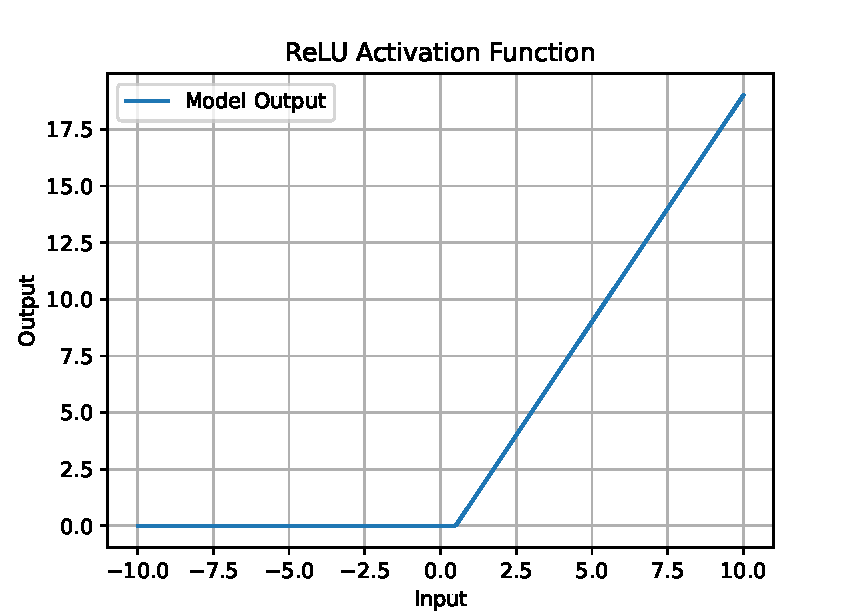
\includegraphics[width=0.6\textwidth]{../Problem 7/MLP_ReLU_plot.pdf}
	\caption{Plot of the MLP using the ReLU activation function}
\end{figure}
\vspace{5mm}


 

